	\section{Prédiction des temps de parcours}

	Le temps de parcours d’un camion sur un chemin varie de manière stochastique, et peut être influencé par divers facteurs tels que l’état de la route ou la météo. Il est important d'être en mesure d'estimer correctement ces temps de parcours afin de bien planifier les opérations. Dans cette section, vous étudierez trois formules qui peuvent être utilisées pour estimer les temps de parcours. 
	
	Lorsqu'un camion débute un trajet, la formule de prédiction estime son temps de parcours. Il s'agit du \textit{temps de parcours prédit}. Lorsque le camion arrive à sa destination, son \textit{temps de parcours observé} est enregistré. Dams le simulateur, le graphe \textit{Temps de parcours observés et prédits} affiche les temps observés et prédits des camions sur plusieurs chemins spécifiques (la légende indique de quels chemins il s'agit).
	
	
	Soient $t_{ij}^k$ et $t^{*k}_{ij}$ les temps prédits et observés pour le segment (chemin) $(i,j)$ à l'instant $k$. $t_{ij}^{k-1}$ et $t^{*k-1}_{ij}$ dénotent les temps prédits et observés du dernier camion sur le segment $(i, j)$ à être arrivé avant l'instant $k$. Soit $A$ l'ensemble des segments. Le logiciel de simulation propose les trois formules suivantes pour estimer le temps de parcours d’un camion sur le segment $(i,j)$ : 
	
	
	\begin{itemize}
		
		\item Moyenne des observations précédentes (sur le même segment)
		
		\begin{equation}
		t_{ij}^k = \frac{1}{n} \sum\limits_{k=1}^n t_{ij}^{*k-1}
		\end{equation}
		
		\item Combinaison convexe
		
		\begin{equation}
		t_{ij}^k = \lambda t^{*k-1}_{ij} + (1-\lambda) t_{ij}^{k-1} \qquad \lambda \in [0, 1]
		\end{equation}
		
		\item Erreur précédente
		
		\begin{equation}
		t_{ij}^k = \lambda t^{*k-1}_{ij} + (1-\lambda) t_{ij}^{k-1} \left( 1- \frac{\sum\limits_{(l,m) \in A} t_{lm}^{k-1} - t_{lm}^{*k-1}}{\sum\limits_{(l,m) \in A} t_{lm}^{*k-1}}\right)
		\end{equation}
		
		
	\end{itemize}
	
	L'interface permet de modifier les valeurs de $n$ et $\lambda$ pour chaque formule.
	
	\vspace{10pt}
	\noindent \textbf{\Large Protocole expérimental: }
	
	\begin{itemize}
		\item Mine : 4 pelles
		\item Nombre de camions de 60 tonnes : 20
		\item Nombre de camions de 100 tonnes : 0
		\item Temps de simulation : 24h
		\item Fonction de score : « aléatoire » (option par défaut)
	\end{itemize}
	
	\vspace{10pt}
	\noindent \textbf{\large Étapes de simulation :  }
	
	\begin{enumerate}
		\item Lancer la simulation à l’aide du bouton play (pour voir l’animation).
		\item Attendre au moins 3h de simulation (pour que les formules de prédictions se stabilisent).
		\item Varier la température (de neige à soleil, ou l’inverse).
		\item Attendre que la formule de prédiction se stabilise de nouveau, ou la fin de la simulation.
	\end{enumerate}
	
	
	
	\subsection{Caractéristiques d'une "Bonne" fonction de prédiction }

 	Les trois fonctions ci-dessus adaptent leurs prédictions en se basant sur les observations précédentes. Donnez deux comportements désirables d'une formule de prédiction.

	\begin{comment}
	\textbf{Réponse : }
	
	\begin{itemize}
		\item Bonne valeur de prédiction en régime stable.
		\item S'adapte rapidement aux changements de conditions.
		\item Peu sensible aux données aberrantes (ex. si un camion tombe en panne).
	\end{itemize} 
	\end{comment}
	%L’objectif est de trouver une formule de prédiction qui réagit rapidement lors de changements drastiques des conditions de conduites sur l’ensemble de la mine.
	
	
	
	
	
	
	\subsection{Étude des formules}
	\label{sec:pred:etude}
	\begin{enumerate}[a)]
		\item Observez le comportement de la formule « Moyenne des observations précédentes » avec différentes valeurs de $n$. Quels sont les avantages et les inconvénients à utiliser une plus grande valeur de $n$. 
		\item En utilisant la formule « combinaison convexe », on observe que plus la valeur de $\lambda$ est grande, plus la formule s’adapte rapidement aux changements de température. Doit-on conclure qu’il vaut mieux utiliser $\lambda=1$? Pourquoi?
		\item La formule « Erreur précédente » est celle qui s’adapte le plus rapidement aux changements de conditions météorologiques. Comment expliquez-vous ce phénomène? 
		\item Si d’autres facteurs que la météo affectaient le temps de déplacement (par exemple, la détérioration soudaine d'une route), la formule "erreur précédente" serait-elle encore valide? Justifiez.
		\item En général, les formules de prédiction semblent plus précises sur le chemin \textit{concentrateur:pelle1} que sur le chemin \textit{sterile:pelle3}. Comment expliquez-vous cela?	
	\end{enumerate}

	\red{Dans la version précédente, la question \ref{sec:pred:etude} était séparée en quatre questions.}	
	
	\subsection{Temps avant le début du remplissage}
	
	Pour cette question, supposez que les temps de transport et de remplissage sont déterministes. Supposons que $n$ camions sont en route pour la pelle et que $m$ camions sont déjà en attente à celle-ci. Soit $t_i$ le temps que prend le camion $i$ pour arriver à la pelle, en secondes, et supposons que les camions sont ordonnés par ordre de temps d'arrivée à la pelle ($t_1 \leq t_2 \leq ...\leq t_{n-1} \leq t_n$). Un camion est en cours de remplissage, et ce remplissage sera complété dans $t^r$ secondes. Le temps de remplissage d'un camion est de $T^R$ secondes. Cette situation est illustrée sur la figure \ref{fig:file}.
	
	\begin{figure}
		\center
		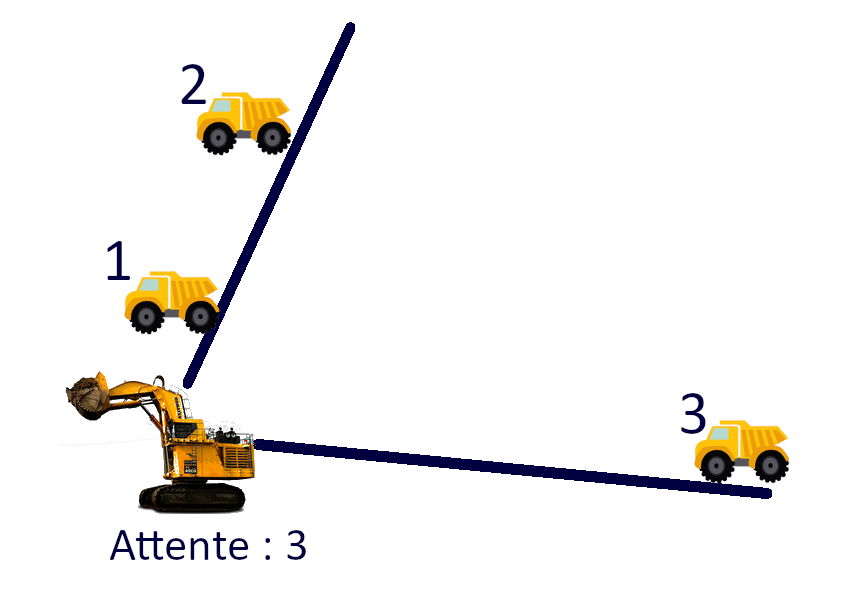
\includegraphics[width=0.4\linewidth]{File.png}
		\caption{\label{fig:file}}
	\end{figure}
	
	Donnez une formule permettant de calculer dans combien de temps débutera le remplissage du camion $n$.
	
	\textbf{Indice :} Il peut s'agir ou non d'une fonction définie par récurrence.
	